\documentclass{article}

\usepackage[margin=1in]{geometry}
\usepackage[colorlinks,linkcolor=blue,filecolor=blue,citecolor=magenta,urlcolor=blue]{hyperref}
\usepackage{bm,amsmath,amsthm,amssymb,multicol,algorithmic,algorithm,enumitem,graphicx,subfigure}
\usepackage{xargs}
\usepackage{natbib}
\usepackage{stmaryrd}


\def\M{\mathcal{M}}
\def\A{\mathcal{A}}
\def\Z{\mathcal{Z}}
\def\S{\mathcal{S}}
\def\D{\mathcal{D}}
\def\R{\mathcal{R}}
\def\P{\mathcal{P}}
\def\K{\mathcal{K}}
\def\E{\mathbb{E}}
\def\F{\mathfrak{F}}
\def\l{\boldsymbol{\ell}}

\newtheorem{Fact}{Fact}
\newtheorem{Lemma}{Lemma}
\newtheorem{Prop}{Proposition}
\newtheorem{Theorem}{Theorem} 
\newtheorem{Def}{Definition}
\newtheorem{Corollary}{Corollary}
\newtheorem{Conjecture}{Conjecture}
\newtheorem{Property}{Property}
\newtheorem{Observation}{Observation}
\newtheorem{Exa}{Example}
\newtheorem{assumption}{H\!\!}
\newtheorem{Remark}{Remark}
\newtheorem*{Lemma*}{Lemma}
\newtheorem*{Theorem*}{Theorem}
\newtheorem*{Corollary*}{Corollary}
 
\newcommand{\eqsp}{\;}
\newcommand{\beq}{\begin{equation}}
\newcommand{\eeq}{\end{equation}}
\newcommand{\eqdef}{\mathrel{\mathop:}=}
\def\EE{\mathbb{E}}
\newcommand{\norm}[1]{\left\Vert #1 \right\Vert}
\newcommand{\pscal}[2]{\left\langle#1\,|\,#2 \right\rangle}
\def\major{\mathsf{M}}
\def\rset{\ensuremath{\mathbb{R}}}


\begin{document}



\title{AniLA: Anisotropic Langevin Dynamics for training Energy-Based Models}

 \author{\textbf{Belhal Karimi, Jianwen Xie, Ping Li} \\\\
 Cognitive Computing Lab\\
 Baidu Research\\
   10900 NE 8th St. Bellevue, WA 98004, USA
 }

\date{}
\maketitle

\begin{abstract}
We develop in this paper
\end{abstract}

\section{Introduction}
The modeling of a data generating process is critical for many tasks.
A growing interest in generative models within the realm of computer vision has led to multiple interesting solutions.
In particular, Energy Based Models (EBM) \citep{zhu1998filters,lecun2006tutorial}, are a class of generative models that learns high dimensional and complex (in terms of landscape) representation/distribution of the input data.
Since inception, EBMs have been used in several applications including computer vision \citep{ngiam2011learning, xie2016theory,xie2020generative,du2019implicit}, natural language processing \citep{mikolov2013distributed,deng2020residual},  density estimation \citep{wenliang2019learning,song2020sliced} and reinforcement learning \citep{haarnoja2017reinforcement}.

Formally, EBMs are built upon an unnormalized log probability, called the energy function, that is not required to sum to one, as standard log probability functions.
This noticeable feature allows for more freedom in the way one parametrizes the EBM.
For instance, Convolutional Neural Network (CNN) can be employed to parametrize the energy function, see \citep{xie2016theory}.
Note that this choice is highly related to the type of the input data, as mentioned in \citep{song2021train}.

The training procedure of such models consists of finding an energy function that assigns to lower energies to observations than unobserved points.
This phase can be casted into an optimization task and several ways are possible to achieve it.
In this paper, we will focus on training the EBM via Maximum Likelihood Estimation (MLE) and defer the readers to \citep{song2021train} for alternative procedures.
Particularly, while using MLE to fit the EBM on a stream of observed data, the high non-convexity of the loss function leads to a non closed form maximization step. In general, gradient based optimization methods are thus used during that phase.
Besides, given the intractability of the normalizing constant of our model, the aforementioned gradient, which is an intractable integral, needs to be approximated.
A popular and efficient way to conduct such approximation is to use Monte Carlo approximation where the samples are obtained via Markov Chain Monte Carlo (MCMC).



\section{On MCMC based Energy Based Models}

Given a stream of input data noted $x \in \rset^p$, the energy-based model (EBM) is a Gibbs distribution defined as follows:
\beq\label{eq:ebm}
p_{\theta}(x) = \frac{1}{Z(\theta)} \mathrm{exp}(f_{\theta}(x))
\eeq

where $\theta \in \rset^d$ denotes the global vector parameters of our model and $Z(\theta) \eqdef \int_{x} \mathrm{exp}(f_{\theta}(x)) \textrm{d}x$ is the normalizing constant (with respect to $x$).




\paragraph{Energy Based Models: }
Energy based models \cite{lecun2006tutorial,ngiam2011learning} are a class of generative models that leverages the power of Gibbs potential and high dimensional sampling techniques to produce high quality synthetic image samples.
Training of such models occurs via Maximum Likelihood (ML).

\paragraph{MCMC procedures: }
MCMC are a class of inference algorithms



\section{Gradient Informed Langevin Diffusion}

\subsection{Preliminaries and Bottlenecks of Langevin MCMC based EBM}
State of the art MCMC sampling algorithm, particularly used during the training procedure of EBMs, is the discretized Langevin diffusion, casted as Stochastic Gradient Langevin Dynamics (SGLD), see \cite{welling2011bayesian}.

\subsection{Curvature informed MCMC}

We introduce a new sampler based on the Langevin updates presented above.

\begin{algorithm}[H]
\caption{\algo for Energy-Based Model} \label{alg:anila}
\begin{algorithmic}[1]
%\small
\STATE \textbf{Input}: Total number of iterations $T$, number of MCMC transitions $K$ and of samples $M$ learning rate $\eta$, initial values $\theta_0$, initial chain states $\{ z_{0}^m \}_{m=1}^M$ and $n$ observations $\{ x_{i} \}_{i=1}^n$.
\FOR{$t=1$ to $T$}
\STATE Compute the anisotropic stepsize as follows: \label{line:step}
\beq
\stepsize_t = \frac{b}{\max(b, | \nabla f_{\theta_t}(z_{t-1}^m) |}
\eeq
\STATE Draw $m$ samples $\{ z_{t}^m \}_{m=1}^M$ from the objective potential \eqref{eq:ebm} via Langevin diffusion:\label{line:langevin}
\beq
z_{t}^{m} = z_{t-1}^m + \stepsize_t/2  \nabla f_{\theta_t}(z_{t-1}^m) + \sqrt{\stepsize} \mathsf{B}_t
\eeq
where $\mathsf{B}_t$ is the brownian motion, drawn from a Normal distribution.
\STATE Samples $m$ positive observations $\{ x_{i} \}_{i=1}^m$ from the empirical data distribution.
\STATE Compute the gradient of the empirical log-EBM \eqref{eq:ebm} as follows:
\beq
\nabla \sum_{i=1}^m \log p_{\theta_t}(x_i) = \mathbb{E}_{p_{\text {data }}}\left[\nabla_{\theta} f_{\theta_t}(x)\right]-\mathbb{E}_{p_{\theta}}\left[\nabla_{\theta_t} f_{\theta}(z_t^m)\right] \approx \frac{1}{m} \sum_{i=1}^{m} \nabla_{\theta} f_{\theta_t}\left(x_{i}\right)-\frac{1}{m} \sum_{i=1}^{m} \nabla_{\theta} f_{\theta_t}\left(z_t^m\right)
\eeq
\STATE Update the vector of global parameters of the EBM:
\beq
\theta_{t+1} = \theta_{t+1} + \eta \nabla \sum_{i=1}^m \log p_{\theta_t}(x_i)
\eeq
\ENDFOR
\STATE \textbf{Output:} Generated samples $\{ z_{T}^m \}_{m=1}^M$
\end{algorithmic}
\end{algorithm}



\section{Geometric ergodicity of AniLA sampler}
We will present in this section, our theoretical analysis for the Markov Chain constructed using Line~\ref{line:step}-\ref{line:langevin}. 

Let $\Theta$ be a subset of $\rset^d$ for some integer $d >0$.
We denote by $\zset$ the measurable space of $\rset^\ell$ for some integer $\ell >0$.
We define a family of stationary distribution $\left(\pi_\theta(z) \right)_{\theta \in \Theta}$, probability density functions with respect to the Lebesgue measure on the measurable space $\zset$. This family of p.d.f. defines the stationary distributions of our newly introduced sampler.

\textbf{Important Note:} The stationary distributions are defined per $\theta \in \Theta$, \ie at each model update during the EBM optimization phase.

For any chain state $z \in \zset$ we denote by $\Pi_\theta(z,\cdot)$ the transition kernel as defined in the \algo update in Line~\ref{line:langevin}.

The objective of this section is to rigorously show that each transition kernel $\pi_\theta$ is uniformly geometrically ergodic and that this result is true uniformly in state $s$ on any compact subset $\mathcal{C} \in \zset$.
As a background note, a Markov chain, as built Line~\ref{line:langevin}, is said to be geometrically ergodic when $k$ iterations of the same transition kernel is converging to the stationary distribution of the chain and this convergence as a geometric dependence on $k$.

We begin with several usual assumptions for such results.
The first one is related to the continuity of the gradient of the log posterior distribution and the unit vector pointing in the direction of the sample $z$ and the unit vector pointing in the direction of the gradient of the log posterior distribution at $z$:
\begin{assumption}\label{ass:cont}
(Continuity) The stationary distribution is positive and has continuous derivative such that for all $\theta \in \rset^d$:
\begin{equation}
\lim \limits_{z \to \infty} \frac{z}{|z|} \nabla f_{\theta}(z) = - \infty \quad \textrm{and} \quad \lim \sup \limits_{z \to \infty} \frac{z}{|z|} \frac{\nabla f_{\theta}(z) }{|\nabla f_{\theta}(z) |} < 0
\end{equation}
\end{assumption}

We assume also some regularity conditions of the stationary distributions with respect to state $s$:
\begin{assumption}\label{ass:contlogpi}
For all $z \in \zset$, $\theta \to \pi_\theta$ and $\theta \to \nabla \log \pi_\theta$ are continuous on $\Theta$.
\end{assumption}

For a positive and finite function noted $V: \zset \mapsto \rset$, we define the V-norm distance between two arbitrary transition kernels $\Pi_1$ and $\Pi_2$ as follows:

\beq
\| \Pi_1 - \Pi_2 \|_V \eqdef \sup \limits_{z \in \zset} \frac{\| \Pi_1(z, \cdot) - \Pi_2(z, \cdot) \|_V }{V(z)}
\eeq

The definition of this norm will allow us to establish a convergence rate for our sampling method by deriving an upper bound of the quantity $\| \Pi_\theta^k - \pi_\theta \|_V$ where $k$ denotes the number of MCMC transitions.
We also recall that $\Pi_\theta$ is the transition kernel defined by Line~\ref{line:langevin} and $\pi_\theta$ is the stationary distribution of our Markov chain. 
Then, this quantity characterizes how close to the target distribution, our chain is getting after a finite time of iterations and will eventually formalize \emph{V-uniform ergodicity} of our method.
We specify that strictly speaking $\pi_\theta$ is a probability measure, and not a transition kernel. However $\| \Pi_\theta^k - \pi_\theta \|_V$ is well-defined if we consider the the probability $\pi_\theta$ as a kernel by making the definition:

\beq
\pi(z, \mathcal{C}) \eqdef \pi(\mathcal{C}) \quad \textrm{for} \quad \mathcal{C} \in \zset, \quad z \in \zset
\eeq


Here, for some $\beta \in ] 0,1[$ we define the V function for all $z \in \zset$ as follows: 
\beq
V_\theta(z) = c_\theta \pi_\theta(z)^{-\beta}
\eeq
where $c_\theta$ is a constant, with respect to the chain state $s$, such that for all $z \in \zset$, $V_\theta(z) \geq 1$.
Again, we note that the V norm is, in our case, function of the chain state noted $z$ \emph{and} of the global model parameter $\theta$, estimated, and thus varying, through the optimization procedure.
The convergence rate will thus be given for a particular model estimate (the supremum in fact).
Define $V_1(z) \eqdef \inf \limits_{\theta \in \Theta} V_\theta(z)$ and $V_2(z) \eqdef \sup \limits_{\theta \in \Theta} V_\theta(z)$ and assume that:

\begin{assumption}\label{ass:V2}
There exists a constant $a_0 > 0$ such that for all $\theta \in \Theta $ and $z \in \zset$, $V_2(z)$ is integrable against the kernel $\Pi_\theta(z, \cdot)$ and 
\beq
 \lim \sup  \limits_{a \to 0}  \sup \limits_{\theta \in \Theta, z \in \zset} \Pi_\theta V_2^a(z) = 1
\eeq
\end{assumption}


We will now give the main convergence result of our sampling method in \algo.
The result consists of showing V-uniform ergodicity of the chain, the irreducibility of the transition kernels and their aperiodicity, ssee \cite{meyn2012markov} for more details. 
We also prove a drift condition which states that the transition kernels tend to bring back elements into a small set from which boils down V-uniform ergodicity of the transition kernels $(\Pi_\theta)_{\theta \in \Theta}$.


\begin{Theorem}
Assume H\ref{ass:cont}-H\ref{ass:V2}.

\end{Theorem}

\clearpage
\section{Numerical Experiments}

\subsection{Application on Toy Example: Gaussian Mixture Model}

\begin{figure}[H]
\begin{center}
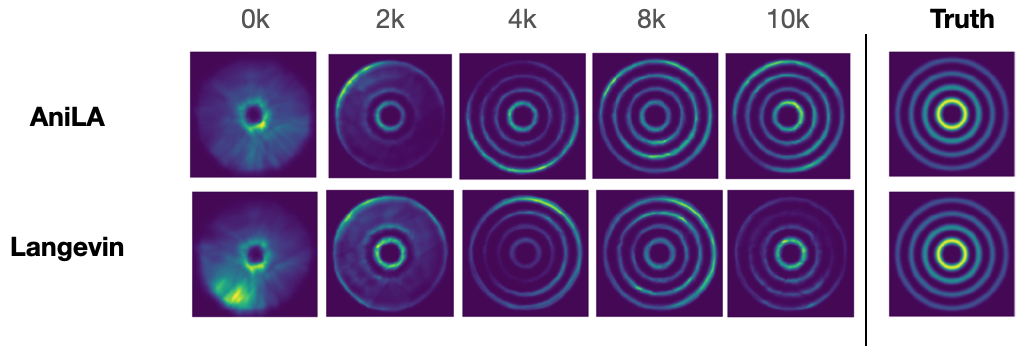
\includegraphics[width=0.8\textwidth]{figs/rings}
\caption{(Rings Toy Dataset) }
\label{fig:results}
\end{center}
\end{figure}


\subsection{Flowers Dataset}

\begin{figure}[H]
    \begin{center}
        \mbox{
        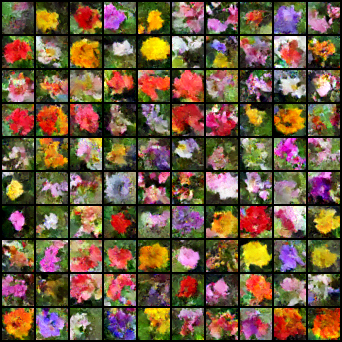
\includegraphics[width=2in]{figs/flowerslangevin}
        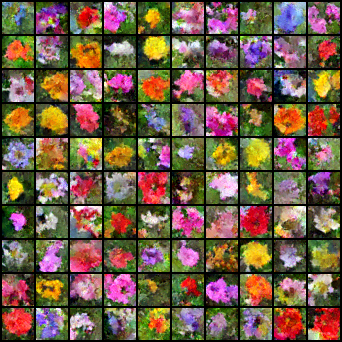
\includegraphics[width=2in]{figs/flowersanila}
        }
    \end{center}
    \vspace{-0.1in}
	\caption{(Flowers Dataset). Left: Langevin Method. Right: AniLA method. After 100k iterations.}
	\label{fig:flowers}
\end{figure}

\subsection{CIFAR Dataset}



\begin{figure}[H]
    \begin{center}
        \mbox{
        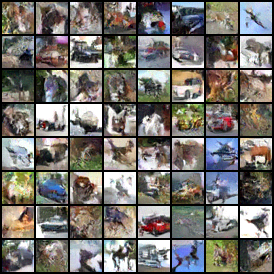
\includegraphics[width=2in]{figs/cifarlangevin}
        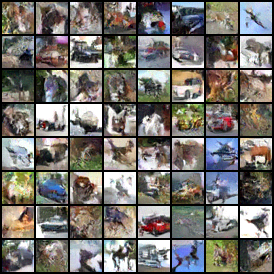
\includegraphics[width=2in]{figs/cifarlangevin}
        }
    \end{center}
    \vspace{-0.1in}
	\caption{(CIFAR Dataset). Left: Langevin Method. Right: AniLA method. After 100k iterations.}
	\label{fig:cifar}
\end{figure}


\section{Conclusion}

\newpage

\bibliographystyle{plainnat}
\bibliography{ref}


\end{document} 